\section{Compressed Sensing}

\begin{frame}[plain,c]
    %\frametitle{A first slide}
    
    \begin{center}
        \color{DarkBlue}
    \Huge Compressed Sensing
    \end{center}
    
\end{frame}

\begin{frame}{Another look at redundancy: the prior point of view}
    % give a sense of what structure is and how it relates to redundancy
    % Redundancy is not always strict: we may only have a strong correlation between 2 structures of the image.
    Redundancy is not always strict
    \begin{figure}
        \centering
        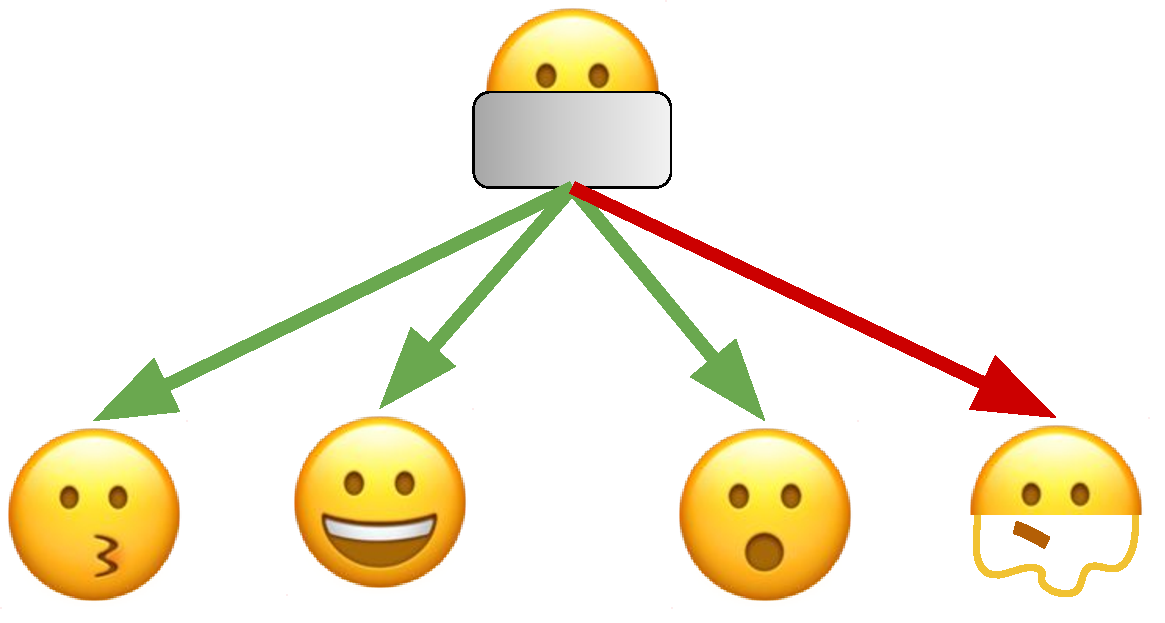
\includegraphics[height=0.5\textheight]{Figures/cs_figures/smiley_prior.pdf}
        \caption{\label{fig:redundancy-smiley}\textbf{A smiley example to a priori knowledge.} 
        % Even if we do not have access to the whole image, we still know which images are more \emph{likely} to correspond to it.
        }
    \end{figure}
\end{frame}

\subsection{Linear Inverse Problems}
\begin{frame}{Linear Inverse Problems}
    % introduce linear inverse problems
    % To leverage this type of redundancy, we introduce the concept of \textbf{Linear Inverse Problems}:
    \textbf{Linear Inverse Problems}:
    \begin{equation*}
        \tikzmarknode{A}{\highlight{green}{$\Ab$}} \tikzmarknode{x}{\highlight{blue}{$\xb$}} = \tikzmarknode{y}{\highlight{yellow}{$\yb$}}
    \end{equation*}
    \vspace{2.5\baselineskip}
    \begin{tikzpicture}[overlay,remember picture,>=stealth,nodes={align=left,inner ysep=1pt},<-]
        % XXX: maybe have smiley + explanation
        % For "A"
        % XXX make green darker everywhere
        \onslide<6>{
        \path (A.south) ++ (0,-2em) node[anchor=south east,color=green!77] (exp_A){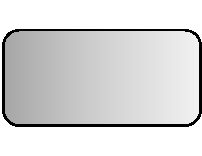
\includegraphics[width=0.05\textwidth]{Figures/intro_figures/smiley_prior_forw_op.pdf}};
        \draw [color=green!87](A.south) |- ([xshift=-0.3ex,color=green]exp_A.south west);
        }
        \onslide<7->{
        \path (A.south) ++ (0,-2em) node[anchor=south east,color=green!77] (exp_A){\textbf{Measurement operator}};
        \draw [color=green!87](A.south) |- ([xshift=-0.3ex,color=green]exp_A.south west);
        }
        % For "x"
        \onslide<2>{
            \path (x.south) ++ (0, -4.5em) node[anchor=south east,color=blue!67] (exp_x){
\includegraphics[width=0.05\textwidth]{Figures/intro_figures/smiley_prior_x.pdf}};
        \draw [color=blue!87](x.south) |- ([xshift=-0.3ex,color=blue]exp_x.south west);
        }
        \onslide<3->{
        \path (x.south) ++ (0, -4.5em) node[anchor=south east,color=blue!67] (exp_x){\textbf{Signal to reconstruct}};
        \draw [color=blue!87](x.south) |- ([xshift=-0.3ex,color=blue]exp_x.south west);
        }
        % For "y"
        \onslide<4>{
            \path (y.south) ++ (0, -1em) node[anchor=north west,color=yellow!67] (exp_y){
\includegraphics[width=0.05\textwidth]{Figures/intro_figures/smiley_prior_y.pdf}};
            \draw [color=yellow!87](y.south) |- ([xshift=-0.3ex,color=yellow]exp_y.south east);
        }
        \onslide<5->{
        \path (y.south) ++ (0, -1em) node[anchor=north west,color=yellow!67] (exp_y){\textbf{Measurements}};
        \draw [color=yellow!87](y.south) |- ([xshift=-0.3ex,color=yellow]exp_y.south east);
        }
    \end{tikzpicture}
    

    \onslide<8->{
    % Problems arise when $\ker{\Ab} \neq \{0\}$, i.e. when there are multiple solutions to this equation.
    Problem: what if $\ker{\Ab} \neq \{0\}$? Multiple solutions!
    }

    \onslide<9->{
    \hfill \break
    % In order to select one of these solutions, we need to use a priori knowledge.
    To select one of these solutions, we need a priori knowledge.
    }
\end{frame}

\begin{frame}{Sparsity and Inverse Problems}
    % explain the concept of sparsity and its link to recovery guarantees
    \begin{definition}[Sparsity]
        A vector $\xb \in \mathbb{C}^n$ is called $s$-sparse if it contains at most $s$ non-zero entries.
    \end{definition}

    \begin{lemma}[Optimization reformulation of sparse vector recovery~\citep{Foucart2013SparseSystems}]
        For a given sparsity $s$, and $s$-sparse vector $\xb$:
    \begin{enumerate}[(a)]
        \item The vector $\xb$ is the unique $s$-sparse solution of $\Ab \xb = \yb$, that is $\{\zb \in \mathbb{C}^n : \Ab \zb = \Ab \xb, \|z\|_0 \leq s\} = \{\xb\}$
        \item The vector $\xb$ can be reconstructed as the unique solution of:
        \begin{equation*}
            \label{eq:cs-problem-l0-min}
            \min_{\zb \in \mathbb{C}^n} \|\zb\|_0 \quad \text{subject to} \quad \Ab \zb = \yb
        \end{equation*}
    \end{enumerate}
    \end{lemma}
\end{frame}

\begin{frame}{Recovery guarantees}
    \begin{theorem}[{{\citep[Theorem~2.13]{Foucart2013SparseSystems}}}]
        The following properties are equivalent:
\begin{enumerate}[(a)]
    \item Every $s$-sparse vector $\xb \in \mathbb{C}^n$ is the unique $s$-sparse solution of $\Ab \zb = \Ab \xb$, that is, if $\Ab \xb = \Ab \zb$ and both $\xb$ and $\zb$ are $s$-sparse, then $\xb = \zb$.
    \item The null space $\ker(\Ab)$ does not contain any $2s$-sparse vector other than the zero.
    \item Every set of $2s$ columns of $\Ab$ is linearly independent.
\end{enumerate}
    \end{theorem}
\end{frame}

\begin{frame}{Application to MRI}
    % MR images themselves cannot be represented as sparse vectors directly, we need a way to express them as such.
    MR images are not sparse as is.
    % \citet{Lustig2007} did that by using the fact that MR images can be represented sparsely in a \textbf{wavelet} basis.
    \citet{Lustig2007} expressed their sparsity in a \textbf{wavelet} basis.

    \hfill \break
    The Inverse Problem becomes:
    \begin{equation*}
        \tikzmarknode{FS}{\highlight{green}{$\left(\Ib_L\otimes {\mathcal{F}}_{\Omega}\right)\Sbb$}} \tikzmarknode{x}{\highlight{blue}{$\xb$}} = \tikzmarknode{y}{\highlight{yellow}{$\ybb$}}
    \end{equation*}
    \begin{tikzpicture}[overlay,remember picture,>=stealth,nodes={align=left,inner ysep=1pt},<-]
        % For "FS"
        \onslide<4>{
        \path (FS.south) ++ (0,-4em) node[anchor=south east,color=green!77] (exp_FS){
            \textbf{$\mathcal{F}_{\Omega}$ : FT on the $\Omega$ set;}\\
            \textbf{$\Sbb=[\Sb_1^H,\ldots, \Sb_L^H]^\top$: the sensitivity maps}\\
            \textbf{per coil}
        };
        \draw [color=green!87](FS.south) |- ([xshift=-0.3ex,color=green]exp_FS.south west);
        }
        \onslide<5>{
        \path (FS.south) ++ (0,-4em) node[anchor=south east,color=green!77] (exp_FS){
            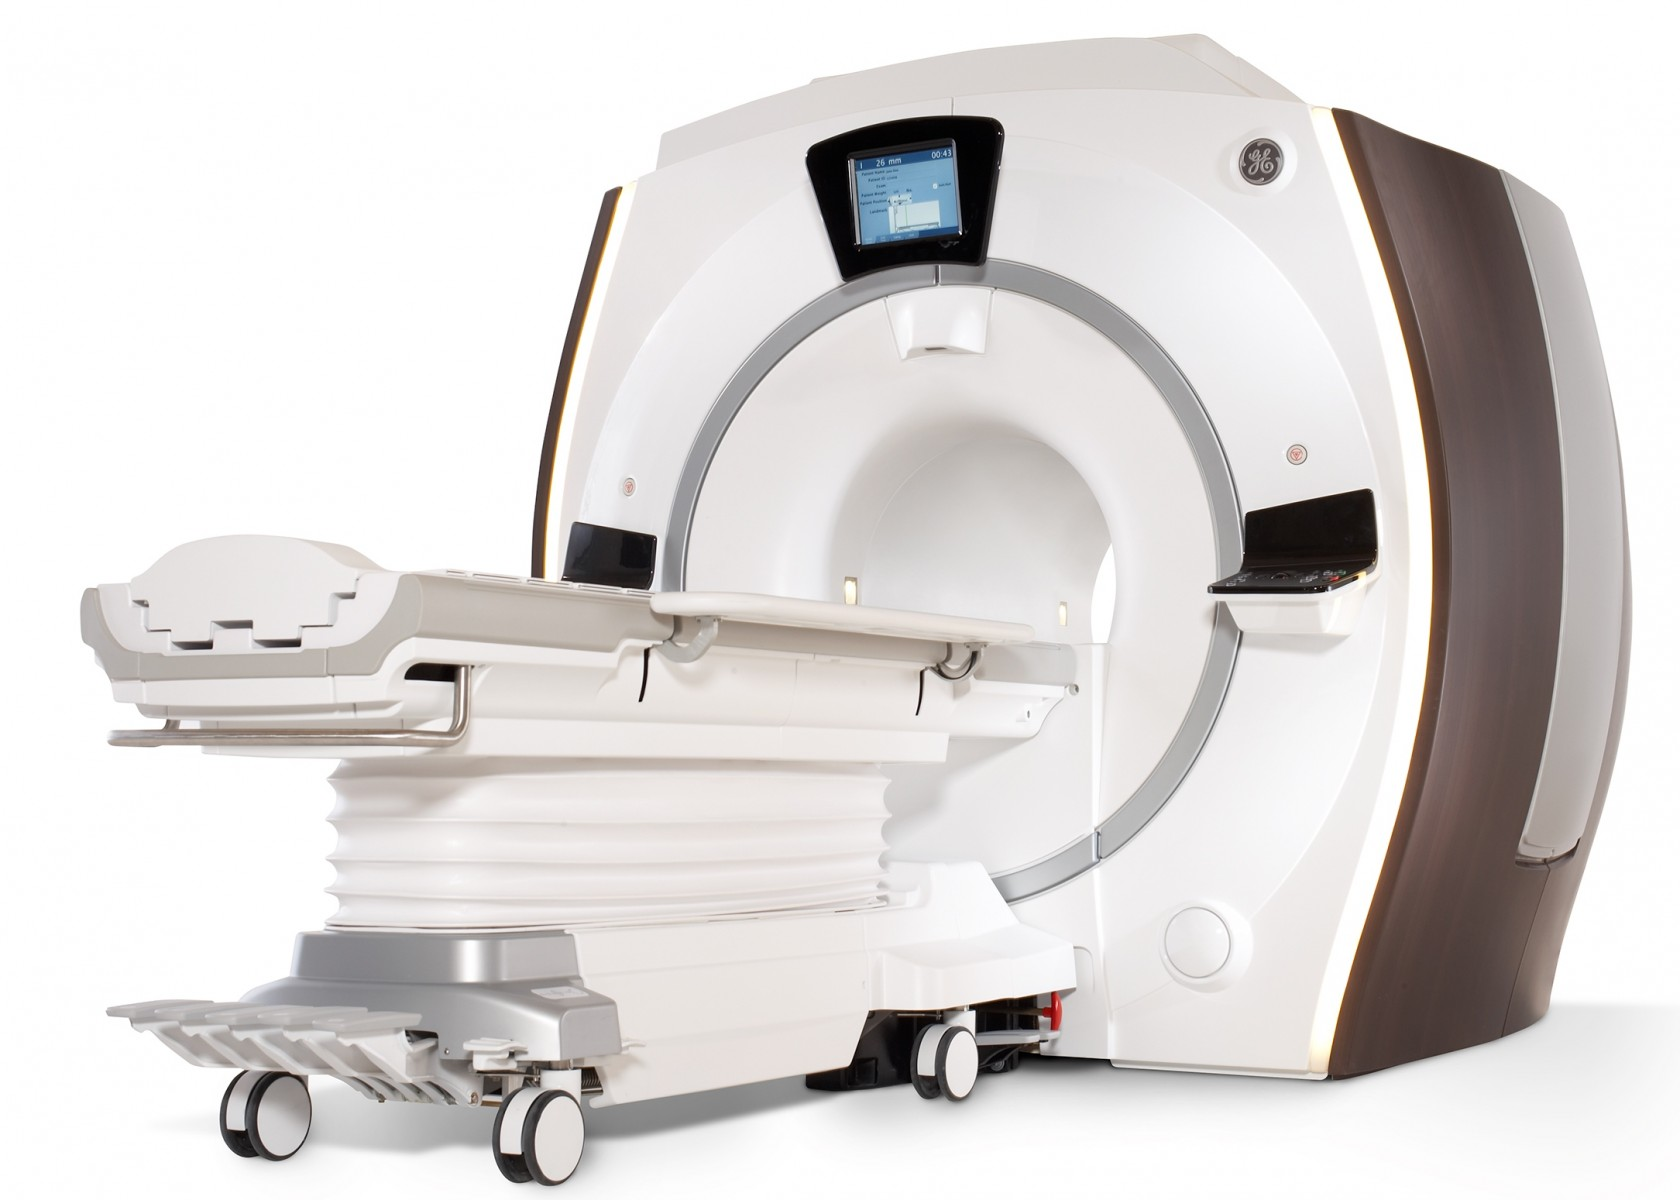
\includegraphics[width=0.1\textwidth]{Figures/intro_figures/mri.jpg}
        };
        \draw [color=green!87](FS.south) |- ([xshift=-0.3ex,color=green]exp_FS.south west);
        }
        % For "x"
        \onslide<2-4>{
        \path (x.south) ++ (0, -2em) node[anchor=south west,color=blue!67] (exp_x){\textbf{2D or 3D MR image}};
        \draw [color=blue!87](x.south) |- ([xshift=-0.3ex,color=blue]exp_x.south east);
        }
        \onslide<5->{
        \path (x.south) ++ (0, -4em) node[anchor=south west,color=blue!67] (exp_x){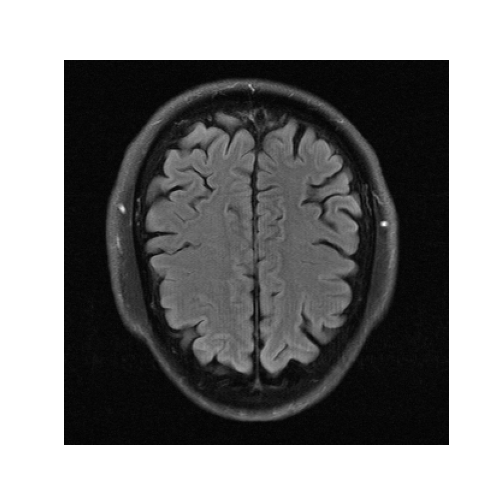
\includegraphics[width=0.1\textwidth]{Figures/intro_figures/brain_mri.png}};
        \draw [color=blue!87](x.south) |- ([xshift=-0.3ex,color=blue]exp_x.south east);
        }
        % For "y"
        \onslide<3-4>{
        \path (y.north) ++ (0, 1em) node[anchor=south west,color=yellow!67] (exp_y){$\ybb=[\yb_1^H, \ldots, \yb_L^H]^\top$,\\ \textbf{k-space measurements} \\ \textbf{for each coil}};
        \draw [color=yellow!87](y.north) |- ([xshift=-0.3ex,color=yellow]exp_y.south east);
        }
        \onslide<5->{
        \path (y.north) ++ (0, 1em) node[anchor=south west,color=yellow!67] (exp_y){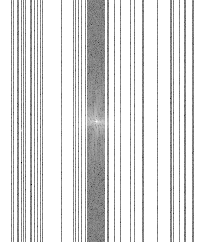
\includegraphics[width=0.07\textwidth]{Figures/intro_figures/kspace_mri.png}};
        \draw [color=yellow!87](y.north) |- ([xshift=-0.3ex,color=yellow]exp_y.south east);
        }
    \end{tikzpicture}
\end{frame}

\subsection{Recovery Algorithms}
\begin{frame}{Relaxation}
    Can we solve the optimization problem?
    \pause
    No; we need to relax it using the basis pursuit:
    \begin{equation*}
        \label{eq:basis-pursuit}
        \min_{\xb \in \mathbb{C}^n} \|\xb\|_1 \quad \text{subject to} \quad \Ab \xb = \yb
    \end{equation*}

    \pause
    % For this problem to have the same solutions as the non-relaxed one, we need coherence-based constraints on the measurement operator $\Ab$.
    Coherence-based constraints on $\Ab$ $\Rightarrow$ same solutions.

\end{frame}

\begin{frame}{The canonical MRI reconstruction problem}
    % We introduce the notion of a \textbf{sparsity} basis $\psib$ (typically wavelets) and the fact that the measurements can be noisy to obtain the canonical MRI reconstruction problem:
    \begin{equation*}
        \min_{\xb \in \mathbb{C}^n} \overbrace{\|\tikzmarknode{calA}{\underline{\mathcal{A}}} \xb - \yb \|_2^2}^{\text{\sf \footnotesize Noisy data consistency}}  + \overbrace{ \tikzmarknode{lambda}{\underline{\lambda}} \|\psib \xb\|_1}^{\text{\sf \footnotesize Regularization term } }
    \end{equation*}
    \vspace{\baselineskip}
    \begin{tikzpicture}[overlay,remember picture,>=stealth,nodes={align=left,inner ysep=1pt},<-]
        % For "calA"
        \path (calA.south) ++ (0,-2.5em) node[anchor=south east,color=black!87] (exp_calA){
            $= \left(\Ib_L\otimes {\mathcal{F}}_{\Omega}\right)\Sbb$
        };
        \draw [color=black!87](calA.south) |- ([xshift=-0.3ex,color=black]exp_calA.south west);
        % For "lambda"
        \path (lambda.south) ++ (0, -2.5em) node[anchor=south west,color=black!87] (exp_lambda){
            Regularization hyperparameter
        };
        \draw [color=black!87](lambda.south) |- ([xshift=-0.3ex,color=black]exp_lambda.south east);
    \end{tikzpicture}
    
\end{frame}

\begin{frame}{ISTA}
    %  The Iterative Shrinkage-Thresholding Algorithm~(ISTA) can be used to solve the canonical MRI reconstruction problem:
     Iterative Shrinkage-Thresholding Algorithm~(ISTA):
     \begin{equation*}
        \label{eq:ista-step}
        \begin{split}
            \xb_{n+1} &= \xb_n - \epsilon_n \mathcal{A}^H\left(\mathcal{A} \xb_n - \ybb\right)\\
            \xb_{n+1} &= \tikzmarknode{prox}{\operatorname{prox}}_{\epsilon_n \tikzmarknode{reg}{\mathcal{R}}}\left(\xb_{n+1}\right)
        \end{split}
    \end{equation*}
    \begin{tikzpicture}[overlay,remember picture,>=stealth,nodes={align=left,inner ysep=1pt},<-]
        % For "prox"
        \path (prox.south) ++ (0,-2.5em) node[anchor=south east,color=black!87] (exp_prox){
            Proximity operator
        };
        \draw [color=black!87](prox.south) |- ([xshift=-0.3ex,color=black]exp_prox.south west);
        % For "reg
        \path (reg.south) ++ (0, -2.5em) node[anchor=south west,color=black!87] (exp_reg){
            \footnotesize $= \|\psib \cdot\|_1$
        };
        \draw [color=black!87](reg.south) |- ([xshift=-0.3ex,color=black]exp_reg.south east);
    \end{tikzpicture}
\end{frame}

% \begin{frame}{Dictionary Learning}

% \end{frame}


\begin{frame}{Limitations of classical recovery algorithms}
    % give max AF
    % also give a sense of the limitations in compute and in prior learning
    Additional acceleration factor on top of PI: 1.5. % from https://www.philips.fr/healthcare/ressources/landing/the-next-mr-wave/compressed-sense
    
    \pause
    The prior knowledge expressed by the wavelet basis (or other basis) is limited: handcrafted and linear.
\end{frame}

\begin{frame}{Compressed Sensing}
    \begin{block}{Recap}
        MRI is slow because of \textbf{relaxation}. 
        
        \pause
        We can use \textbf{redundancy} in many forms to reduce the amount of samples we need in the Fourier space, and therefore the number of relaxations.
        
        \pause
        But we are limited by simple forms of redundancy.
    \end{block}
\end{frame}